
\section{Introduction}


In the previous chapter, we presented an initial modeling for sizing the renewable infrastructure to reduce the carbon emissions of a cloud federation one year operation --- a relatively short duration. Given that the cloud federation will operate for a long term, DC operators needs to be sure of the investments that they will make to avoid wasting money and as well generating more environmental impact with a bad strategy. Furthermore, a planing process is subject to many uncertainties that if not taken into account will decrease the validity and credibility of the solution. 


This chapter will present an extension of the model focusing on the long-term operation of the cloud DCs and the the uncertainties that this sizing process is subject to. First, we will show an evaluation regarding the uncertainties caused by the intermittency of solar irradiation, and what needs to be considered in the modeling to avoid over or under-sizing of the PV panels. We will also present an evaluation if the adoption of wind power could further reduce the cloud footprint, specially for night operations when the sun is not shining. Some data sources provide the information of the grid carbon footprint at time intervals of one hour, and we will show an analysis if this fine-grain value would affect the renewable infrastructure sizing. Second, once built the renewable infrastructure cannot be reduced --- this would imply on destroying/discarding PV panels, batteries and wind turbines, so we need to find another way to deal with the over-sizing that might be caused by the intermittency of renewable infrastructure. Thankfully, there is another part that can be managed to reduce the impact of wrong-sizing: scheduling of the workload. In cloud platform, a significant part of the workload are tasks that does not have a high priorirt and whose execution can be delayed over time, denominated batch tasks --- represents x\% of facebook and \% of google. 


and , in particular: i) climate conditions: the intermittency of renewable sources is a  problem for the renewable energy productions, and the life time of the equipment is decades, therefore the sizing process needs to avoid over and under-sizing; we also evaluate if adding wind power could further reduce the total carbon footprint of the cloud operation, specially during nights; ii) the increase in workload over time: the demand for cloud computing resources to deal with the increasing number of users and requests for applications is evolving year by year, so one needs to take this into account for the sizing process; iii) the different hardware generations over time: every year there is a new CPU processor that has a higher computational performance and may be more power efficient, and the decision of buying more servers to aggregate or replace the current servers of the DCs needs to take into account that producing these new servers also emits carbon.  Once built, it is not feasible to reduce the renewable infrastructure capacity, this would result in demolishing or discarding the PVs, WT and batteries. One possibility is then analyze the flexibility of the workload that is executed by these DCs, for example, some type of tasks may have less lower restrictions regarding the deadline, such as batch tasks (which represents a significant part of the workload of cloud computing DCs), and may be delayed over time. We will evaluate what is the impact in carbon emissions of delaying $\alpha$ percent of the jobs for $\beta$ time slots.

\subsection{Validating sensibility/robustness of the LP to uncertainties}

To evaluate the sensibility to the linear program, we will evaluate it considering different scenarios in terms of solar irradiation, and grid emissions data.

\subsubsection{Uncertainty related to the climate: solar irradiation}

It is considered that a PV lifetime is 30 years. To evaluate the sensibility of the sizing process considering the solar irradiation data, that is intermittent, we perform the sizing process using the solar irradiation from 30 years (1980 to 2009), that is, for each year the corresponding irradiation data is used for the sizing process, generating a total of 30 instances. To isolate only the effect of the solar irradiation in the sizing process, all the other values are fixed for the 30 instances (workload, parameters, \ch{CO2} emissions from using the grid and manufacturing the renewable infrastructure).

In Figure~\ref{fig:pv_boxplots} we present a boxplot with the different values of the optimal sizing for the 30 years regarding the PV dimensioning, and in Figure~\ref{fig:pv_boxplots} regarding the battery dimensioning. We observe a high difference for the PV area for some locations (Canberra, Seoul, Virginia, and the highest difference was in Singapore). From this we can conclude that using solar irradiation just for a single year is not enough to deal with the intermittency of irradiation, and the PV area can be very different depending on the year selected for the sizing process. For the batteries, the difference in the sizing is small because they are used mostly for night computations.


\begin{figure}[H]
  \centering
  {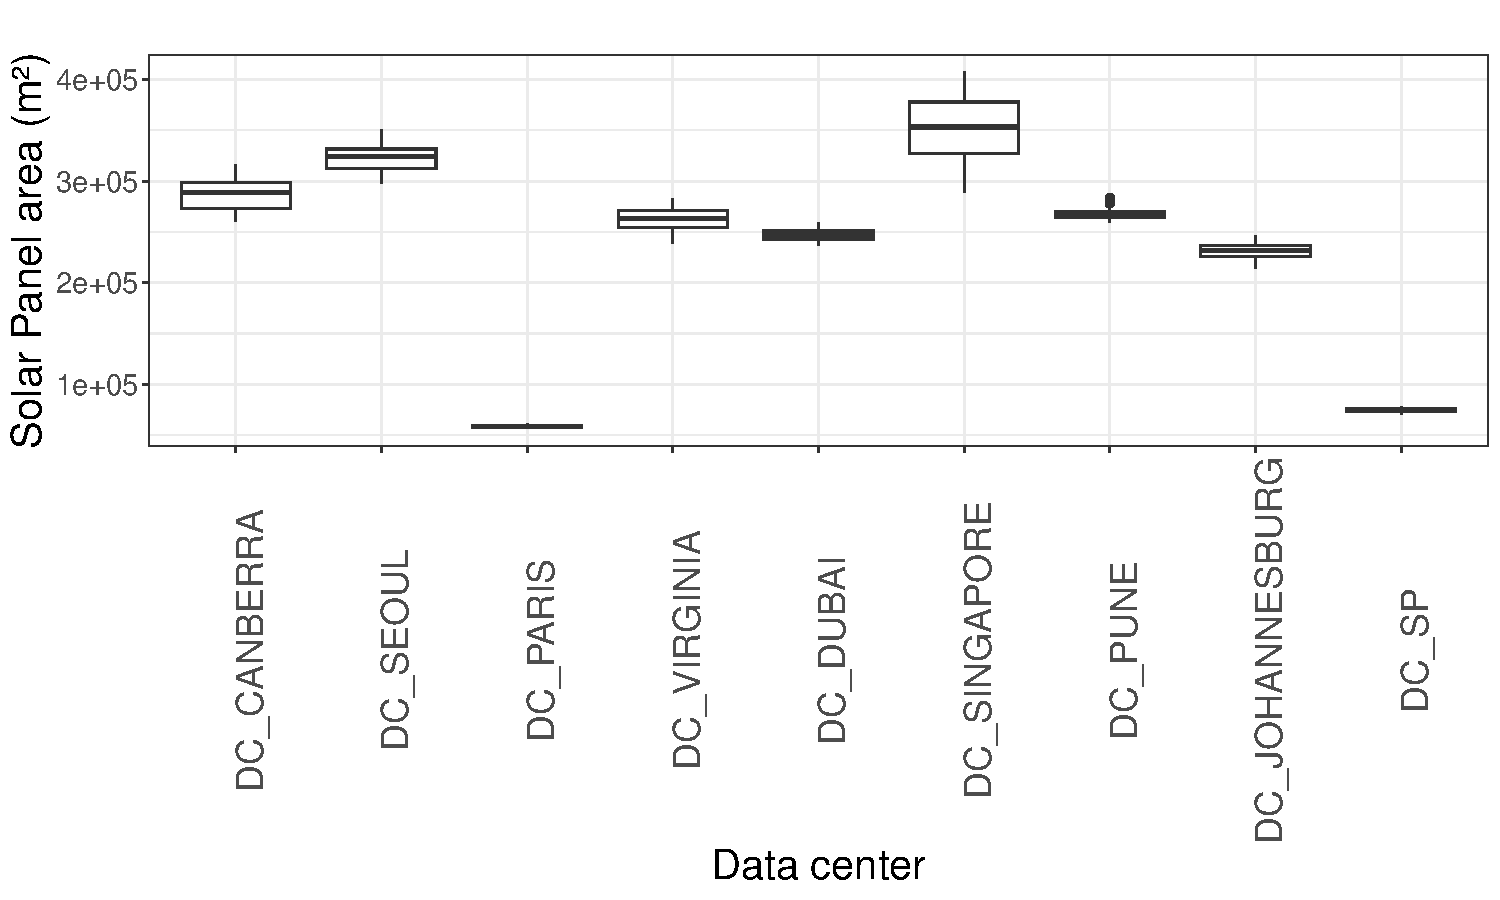
\epsfig{file = images/pv_boxplots_1980_2009.pdf, width = .66\textwidth}}
  \caption{Different PV sizing using irradiation from 30 years (1980 - 2009).}
  \label{fig:pv_boxplots}
\end{figure}


\begin{figure}[H]
  \centering
  {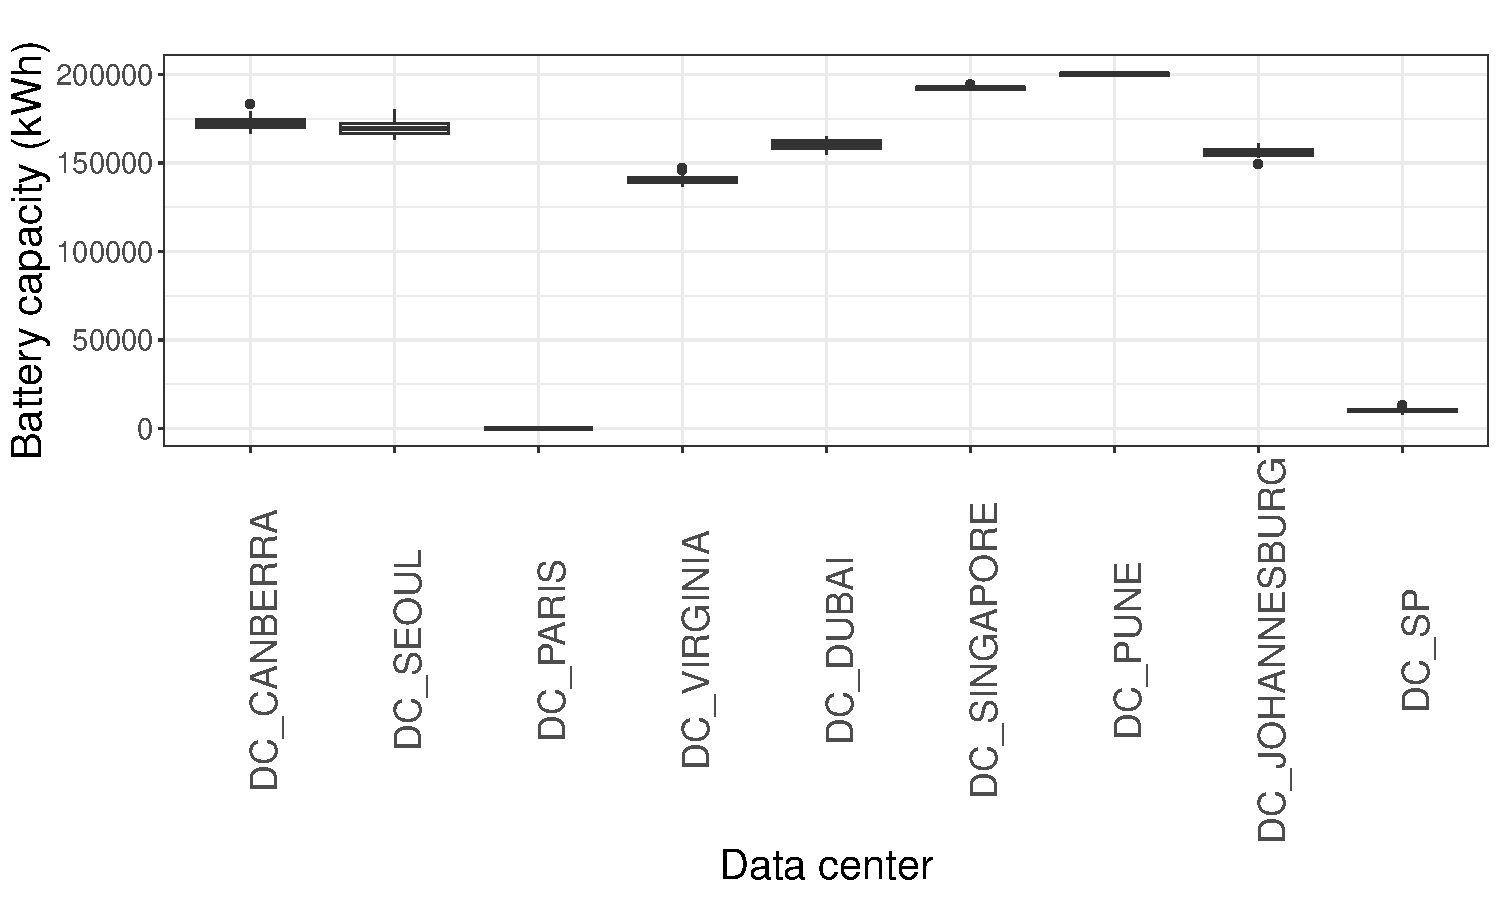
\epsfig{file = images/bat_boxplots_1980_2009.pdf, width = .66\textwidth}}
  \caption{Different battery sizing using irradiation from 30 years (1980 - 2009).}
  \label{fig:bat_boxplots}
\end{figure}


Computing the optimal area of PV and batteries can also be considered as a type of forecasting, given the long life time of the equipments (30 years for PVs and 10 years for batteries) and the uncertainty about the climate conditions during the life time of the renewables infrastructure. In Figure~\ref{fig:pv_boxplots} and Figure~\ref{fig:bat_boxplots}, we showed only the values for the optimal sizing of each year, and when the irradiation is known. The DC operator is interested in the sizing for the future, that is, the following years where the renewable infrastructure will be used. Predicting the solar irradiation data that a region will receive is not a simple task, and it also involves predicting the weather, since clouds can affect the amount of solar irradiation received by the region. 

To evaluate the results of the sizing and which solar irradiation data should be used, we will evaluate it for a duration of 10 years. 
We use the solar irradiation data for 30 years to generate the sizing (from 1980 to 2009) and evaluate the resulted sizing when operating the cloud federation for the next 10 years (from 2010 to 2019), using the new solar irradiation values.

The sizing process was performed for two scenarios considering the 30 years of solar irradiation data: in the first, the average solar irradiation for each hour, and in the second, using the median.

The baseline, was the optimal sizing for the 10 years (2010 - 2019) where all the solar irradiation data is know in advance.
Table \ref{tab:co2_10y} presents the results in terms of \ch{CO2} emissions. We observe that these simple forecasting techniques already have a good precision value, up to 2\% difference compared to the optimal scenario. Using a simple method is also interesting because of the computational costs of the computation, resulting in a smaller \ch{CO2} footprint for the sizing process by itself.

    \begin{table}
      
      \caption{Emissions (in kt \ch{CO2}-eq) for the different scenarios} \centering
    \label{tab:co2_10y}

      \begin{tabular}{|l|r|r|}
        
        \hline
        
        \textbf{Sizing Scenario} &  \textbf{Emissions } & \textbf{Diff. to baseline (\%) } \\
        \hline
        
        Optimal sizing 2010 - 2019  &       296.367 & - \\
        \hline     

        Average irrad.  1980 - 2009  & 301.237 &  1.62 \\
        \hline

        Median irrad. 1980 - 2009  &        304.489 & 2.66 \\
        \hline 
        
      \end{tabular}  
    \end{table}

  



\subsubsection{Uncertainty related to the climate: wind speed}

In this section, we will evaluate the impact adding other renewable power source: wind turbines, and to what extent they complement the photovoltaic power production to reduce the total emissions of the cloud federation operation, in particular during the night and seasons with lower solar irradiation as the winter. We consider a new variable $WT^d$ that represents how much wind turbines will be built at each DC location. The number of wind turbines (WT) is an integer number (we cannot produce 1.2 WT for example). However, to avoid increasing the computational complexity of the LP by including integer variables, we made a relaxation in our modeling to allow the WT variable to be linear. 

The power production of the $WT^d$ wind turbines at location of data center $d$ at instant $k$ ($Pwt^d_{k}$) is modeled by Equation~\ref{eq:wt_power_prod}, where $V^d_k$ is the wind speed at location of data center $d$ at instant $k$; $Vici$ is the \textit{cut in} wind speed, that is, the wind turbines start producing power when the wind speed is greater or equal to $Vici$; $Vco$ is the \textit{cut out} wind speed, that is, the wind turbines stop producing power when the wind speed is greater than $Vco$; $Pr$ is the WT rated power production in W; and $Vr$ is the speed where the WT starts producing $Pr$ power. This model is based from \cite{HADDAD2021100505}.

\begin{equation} \label{eq:wt_power_prod}
Pwt^d_{k} = WT^d \times \left\{ 
  \begin{array}{ c l }
    0   & \quad \textrm{if } V^d_k \leq Vici \\
    Pr \times \frac{V^d_k - Vici}{Vr - Vici}  & \quad \textrm{if } Vici < V^d_k \leq Vr \\
    Pr  & \quad \textrm{if } Vr < V^d_k \leq Vco \\
    0  & \quad \textrm{if } Vco < V^d_k \\
  \end{array}
\right.
\end{equation}

Similar to the PVs, the carbon emissions of manufacturing WT also depends on the location where the WT is installed: the more wind the region receives through the WT life time, the higher is its power production and the lower is its carbon footprint by kWh. $wtCO2^d$ models the carbon emissions of using WT at the location of data center $d$ by kWh, where $FPwt$ is the carbon emissions of building a WT, and $expectedEwt^d$ is the expected total energy that 1 WT will generate during its lifetime (20 years). Here it is considered that 
during all the life cycle of WT (manufacturing to recycling), it will produce 317.9 tons of \ch{CO2} eq \cite{li2020_wtlca}. To represent the total electricity production $expectedEwt^d$ we considered wind speed data from the last 20 years (1993 to 2022) at each location and used Equation~\eqref{eq:wt_power_prod} to compute the power production. Table~\ref{tab:co2_pv_wt_grid} is an updated version of Table~\ref{tab:carbonfootprint} to illustrate also the emissions of using the wind turbines. Finally, Equation~\eqref{eq:fp_using_wt} models the footprint of using the WT at location of data center $d$ at instant $k$. Regarding the WT parameters, it was considered: $Pr$ = 1.5 MW; $Vr$ = 14 m/s; $Vci$ = 4 m/s; $Vco$ = 25 m/s.
 
\begin{equation} 
   wtCO2^d =  \frac{FPwt}{expectedEwt^d} 
\end{equation}

\begin{table}[H]
\caption{Emissions (in $g\,\ch{CO2}-eq.kWh^{-1}$) for PV usage, WT usage, and using the regular grid. Source for grid emissions: electricityMap, climate-transparency.org.}\label{tab:co2_pv_wt_grid} \centering

  \begin{tabular}{|l|r|r|r|}
    
  \hline

  \textbf{Location} &  \textbf{Grid} & \textbf{PV} & \textbf{WT} \\
  \hline
  Johannesburg & 900.6 & 24.90  & 25.52 \\
  \hline
  Pune & 702.8 & 27.96  & 15.4 \\
  \hline
  Canberra & 667.0 & 29.71 & 52.19\\
  \hline
  Dubai & 530.0  & 24.84 & 22.63 \\
  \hline
  Singapore & 495.0 & 36.19 & 69.4\\
  \hline     
  Seoul & 415.6 & 34.00 & 18.25 \\
  \hline
  Virginia  & 342.8 & 31.71 & 480.1 \\
  \hline
  São Paulo &  61.7 & 27.99 & 32.07 \\
  \hline 
  Paris &  52.6  & 39.93 & 12.7 \\
  \hline  


\end{tabular}  
\end{table}


\begin{equation}\label{eq:fp_using_wt}
   FPwt^d_k =  wtCO2^d \times Pwt^d_{k}\times \Delta t
\end{equation}


Given that we are using an additional renewable power infrastructure, it is also necessary to update the model of the renewable power production on DC $d$ at instant $k$. Equation~\eqref{eq:new_pv_power} and Equation~\eqref{eq:new_renewable_power} models that the renewable power can be originated from both the PVs and WT.

\begin{equation} \label{eq:new_pv_power}
    Ppv^d_{k}= I^d_k \times Apv^d \times \eta_{pv}
\end{equation}


\begin{equation} \label{eq:new_renewable_power}
    Pre^d_{k}= Ppv^d_{k} + Pwt^d_{k}
\end{equation}

Finally, the objective function also needs to be modified in order to include the carbon emissions of using WTs. Equation~\ref{eq:new_obj_co2} models the new objective function.

\begin{equation} \label{eq:new_obj_co2}
\text{minimize }\sum_{k=0}^{K-1} \sum_{d=1}^D ( FPgrid^d_k +  FPpv^d_k +  FPwt^d_k) + \sum_{d=1}^D FPbat^d
\end{equation}

To evaluate the impact of including WT, we compare the sizing for using only PVs and batteries and using PV, batteries and WT. The selected year for climate conditions (solar irradiation and wind speed) is 2022. Table~\ref{tab:total_wind_and_pv_co2} presents the results in terms of total emissions when also considering the wind as renewable, we observe a reduction of approximately 6\% in comparison with the scenario where no WT is used and renewable energy is only produced by the PVs. 


\begin{table}[H]

  \caption{Total emissions (tons of \ch{CO2} for different scenarios }\label{tab:total_wind_and_pv_co2} \centering
  
  \begin{tabular}{|l|r|}
   \hline
    
  \textbf{Scenario} &   \textbf{Total \ch{CO2} emissions (tons)} \\

  \hline
  PV + Bat + WT + Grid  & 27821.1 \\
  \hline
  PV + Bat + Grid       & 29541.7 \\
  \hline

\end{tabular}  
\end{table}

Table~\ref{tab:results_wt} presents the number of WT that need to be built at each location. 


\begin{table}[H]
  
  \caption{Computed number of WT for each location}\label{tab:results_wt} \centering

  \begin{tabular}{|l|r|}
   \hline
    
  \textbf{Location} &   \textbf{Number of WT} \\
  \hline
  Johannesburg & 7.03   \\
  \hline
  Pune  & 6.38 \\
  \hline
  Canberra  & 6.22 \\
  \hline
  Dubai   &  5.63 \\
  \hline
  Singapore & 0.0  \\
  \hline     
  Seoul    & 25.29  \\
  \hline
  Virginia   & 0 \\
  \hline
  São Paulo   & 7.47 \\
  \hline 
  Paris    &    19.95 \\

  \hline  

\end{tabular}  
\end{table}


To assess the impact of including the WT regarding the sizing of both PV and batteries, we present in Figure~\ref{fig:wind_bat} and Figure~\ref{fig:wind_pv}  the dimensioning for both equipment considering and not considering manufacturing WT. 

\begin{figure}[H]
  \centering
  {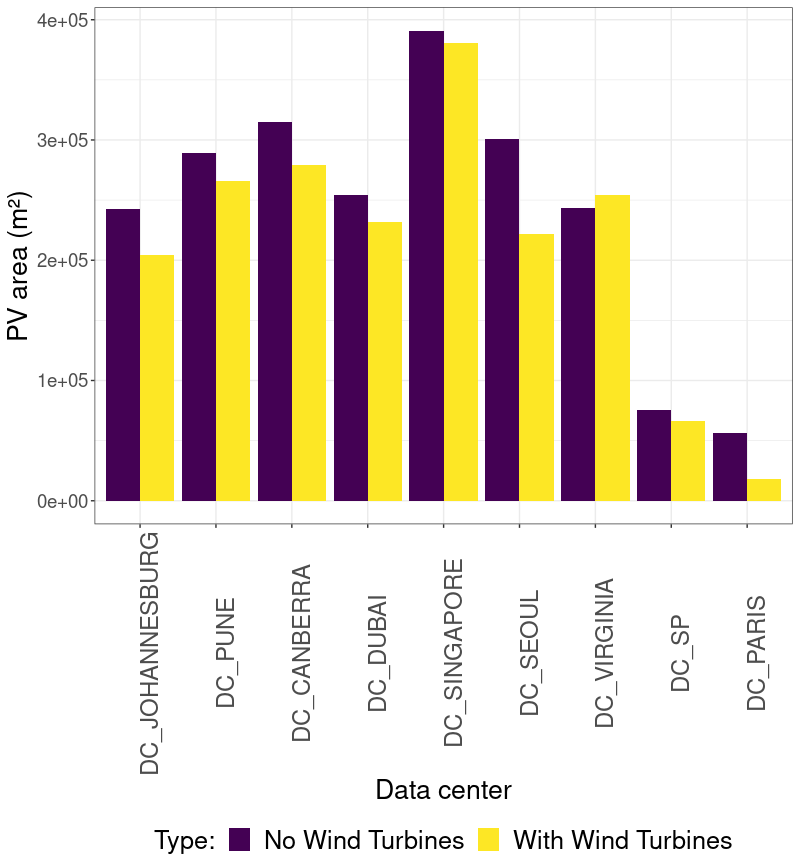
\epsfig{file = images/pv_area_vs_wind_turbines.png, width = .5\textwidth}}
  \caption{PV Area sizing when the WT are and are not included }
  \label{fig:wind_pv}
\end{figure}


\begin{figure}[H]
  \centering
  {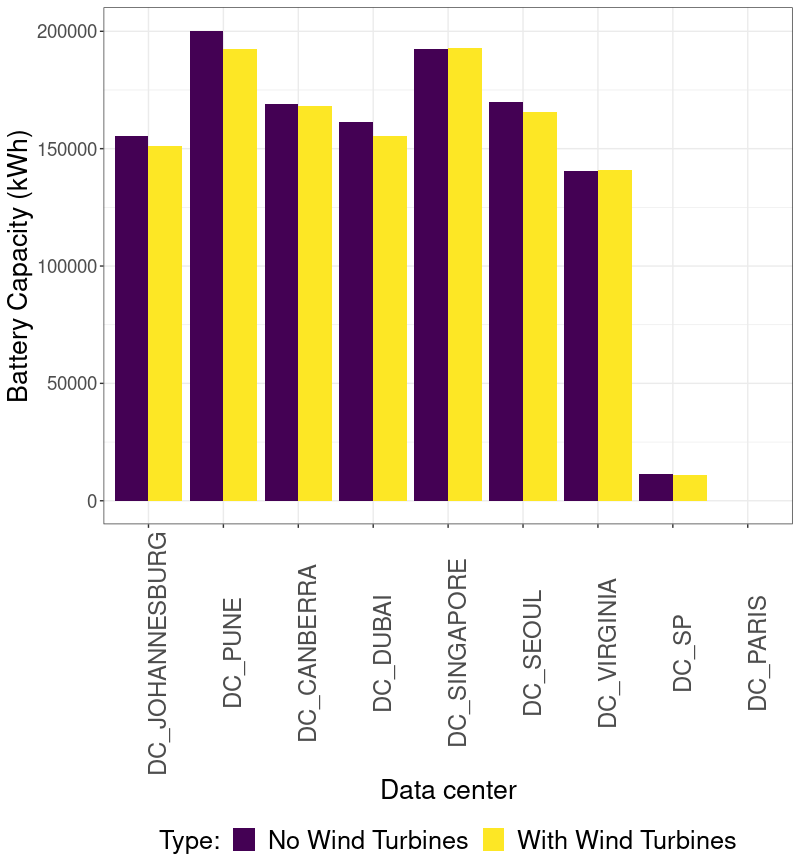
\epsfig{file = images/bat_cap_wind_turbine.png, width = .5\textwidth}}
  \caption{Battery capacity sizing when the WT are and are not included }
  \label{fig:wind_bat}
\end{figure}







\subsubsection{Uncertainty related to the emissions from the local electricity grid }

Given the presence of low-carbon intensive sources in some regions, the emissions of the local electricity grid is not static all over the year, for example, regions that have access to solar energy have a lower grid footprint during the day. Some countries provide access to fine-grain information of its electricity mix in real time or historical data in the form of time series. However, obtaining data for all the locations is not an easy process: not all the locations provide this information, or they provide with different time granularity (day, hour, month), historical data with different spans, or only real time values. Considering the selected locations for the DCs listed before, Table~\ref{tab:grid_emissions_hist} presents the data that was found. 


\begin{table}[H]

  \caption{Comparison of local electricity grid access to information }\label{tab:grid_emissions_hist} \centering
  
  \begin{tabular}{|l|r|r|r|}
   \hline
    
  \textbf{Location} &   \textbf{Granularity} & \textbf{Span} & \textbf{Source} \\
  \hline
  Johannesburg & month & year & ElectricityMaps  \\
  \hline
  Pune  & hour & year & ElectricityMaps  \\
  \hline
  Canberra  & hour &  year & ElectricityMaps \\
  \hline
  Dubai    & year & year & https://1p5ndc-pathways.climateanalytics.org/  \\
  \hline
  Singapore & month & year & ElectricityMaps \\
  \hline     
  Seoul     & hour & year & ElectricityMaps \\
  \hline
  Virginia  &  hour & year & ElectricityMaps \\
  \hline
  São Paulo & hour & year  & ElectricityMaps \\
  \hline 
  Paris     & hour & year  & ElectricityMaps  \\  
  \hline  

\end{tabular}  
\end{table}


In order to evaluate what is the impact of using this fine-grain information of the grid \ch{CO2} on the sizing process, we perform the sizing using the time series provided by Electricity Map for the locations: Pune, Canberra, Seoul, Virginia, São Paulo and Paris. These time series have the span of one year, and one value for each hour. For the regions Johannesburg and Singapore, the information of the \ch{CO2} emissions was in the granularity of months. Therefore, we generated a time series with a total duration of one year with the same value of \ch{co2} per hour for each corresponding month that we have the grid \ch{co2} emissions. For Dubai, we only found data for the year average grid \ch{co2} emissions, and we generated a time series in which the grid emissions is fixed for every hour.


We compared the results of using this fine grain value, with the results of using the average of the grid emissions for the year. Table~\ref{tab:co2_grid_granularities} presents the results. Furthermore, there was an increase of 0.25\% in \ch{CO2} emissions. Figure~\ref{fig:pv_grid_co2_sizing} and \ref{fig:bat_grid_co2_sizing} illustrates the difference in the sizing, both for PVs and batteries, respectively, when we use this different granularity for grid \ch{CO2} emissions data.



\begin{table}[H]

  \caption{Total emissions (tons of \ch{CO2}) for different scenarios }\label{tab:co2_grid_granularities} \centering
  
  \begin{tabular}{|l|r|r}
   \hline
    
  \textbf{Scenario} &   \textbf{Total \ch{CO2} emissions (tons)} \\
  \hline
  Fine grain grid emissions data & 30911.03 \\
  \hline
  Average of the year grid emissions data & 30831.14 \\
  \hline

\end{tabular}  
\end{table}


\begin{figure}[H]
  \centering
  {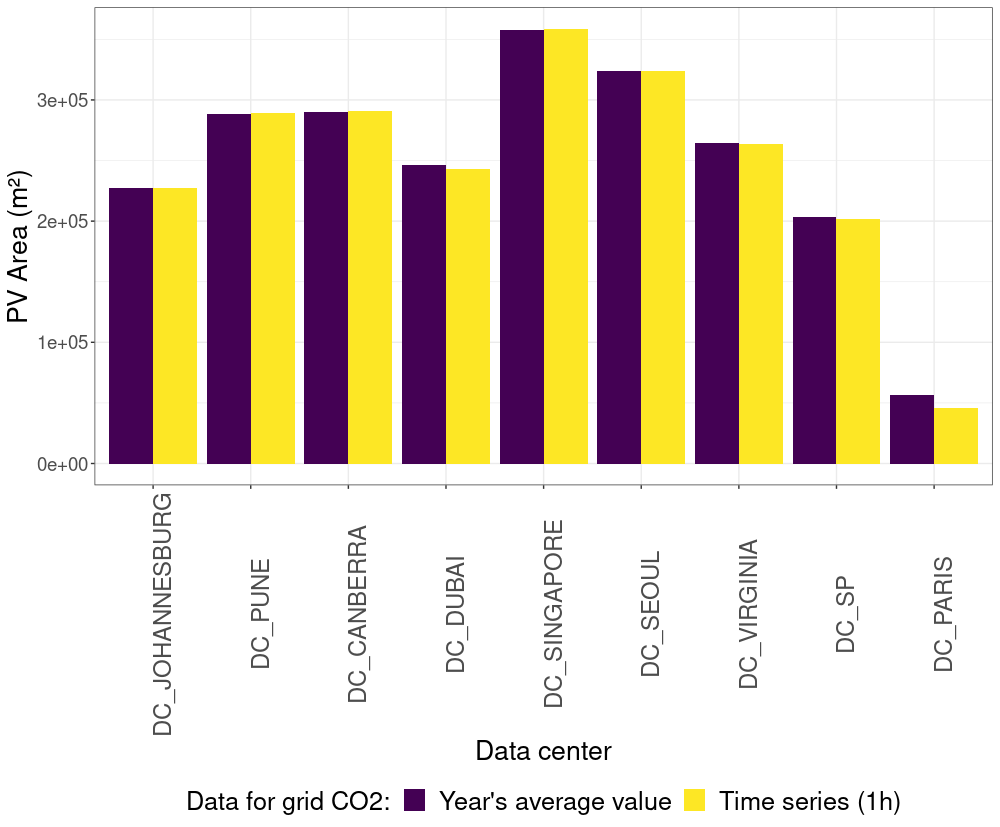
\epsfig{file = images/sizing_pv_grid_co2.png, width = \textwidth}}
  \caption{PV sizing with different granularity for grid \ch{CO2} emissions data}
  \label{fig:pv_grid_co2_sizing}
\end{figure}


\begin{figure}[H]
  \centering
  {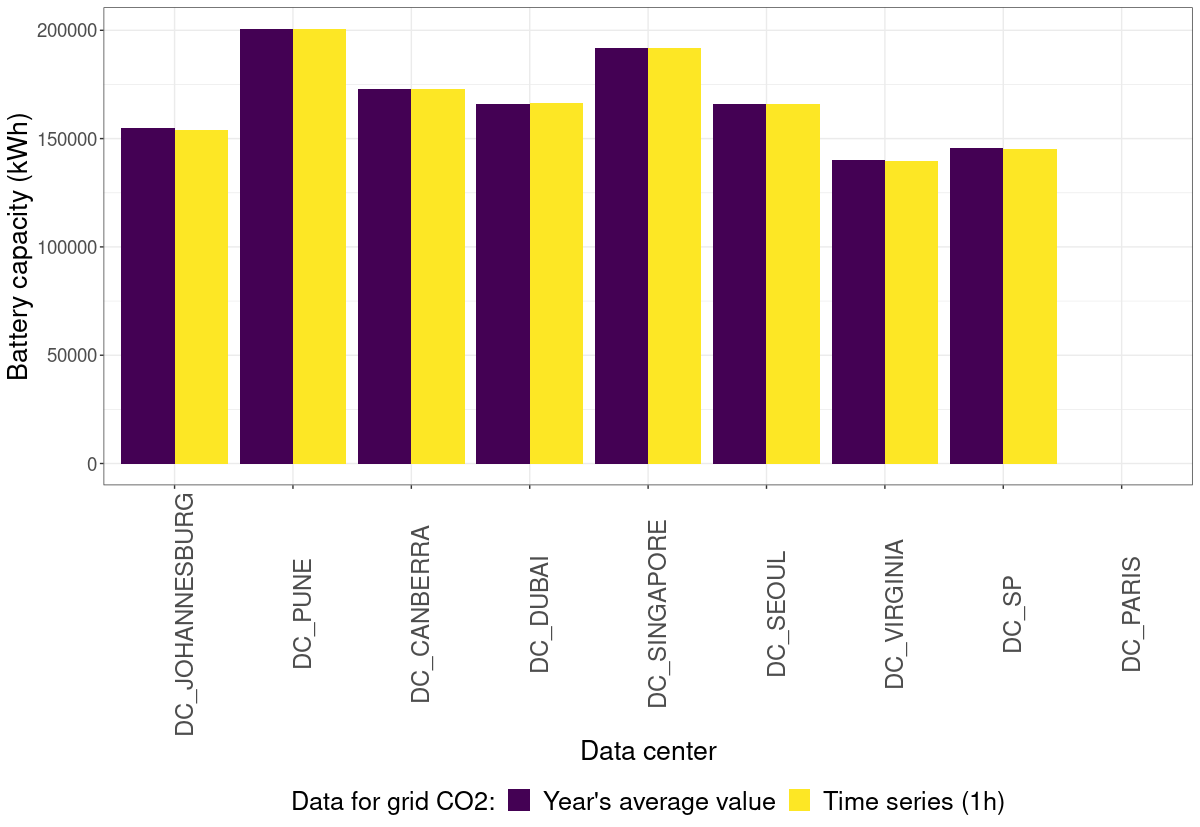
\epsfig{file = images/sizing_bat_grid_co2.png, width = \textwidth}}
  \caption{Battery sizing with different granularity for grid \ch{CO2} emissions data }
  \label{fig:bat_grid_co2_sizing}
\end{figure}





\begin{table}[H]

  \caption{Difference in total emissions (tons of \ch{CO2}) between using avg. co2 of the year vs co2 per hour for the different years. Values greater than zero represents that using co2 values per hour increased the total emissions.}\label{tab:co2_grid_granularities_years} \centering

  \begin{tabular}{|l|r|r}
   \hline
   
  \textbf{Year} &   \textbf{Difference (\%)} \\
  \hline
  2021 &   0.25 \\
  \hline
  2020 &   0.10 \\
  \hline
  2019 & -0.18 \\
  \hline
  2018 & -0.09 \\
  \hline

\end{tabular}  
\end{table}





\subsubsection{Uncertainty related to the workload}

It is expected that the workload of the clouds will keep evolving during the lifetime of the data center. Here, we presents results considering that the workload will keep increasing by 10\% each year. To evaluate this uncertainty in an isolated way, we created new scenarios only increasing the workload, that is all the other inputs and parameters are fixed. The increase was made by time slot, that is, at each time slot, the value of requested cores is increased by 10\%, and this value is limited by the cloud federation total cores capacity.

To evaluate this uncertainty, first we compute the sizing with the base year of 2021 and the original workload, and the results of the sizing (PV area and capacity of batteries) will be our baseline. Then, using the sizing of the baseline (fixed values for PVs area and battery capacity), we run the LP with the new workloads. Table \ref{tab:workload_emissions} illustrates the increase of \ch{CO2} emissions using these new workloads.

\begin{table}[H]
  \caption{Increase in \ch{CO2} emissions considering the evolving workload (values are in \%) }\label{tab:workload_emissions} \centering
  \begin{tabular}{|r|r|}
   \hline
  \textbf{Years} &   \textbf{Increase in emissions}\\
  \hline
  +1 & 4.6 \\
  \hline
  +2  & 14.7  \\
  \hline
  +3  & 19.7 \\  
  \hline  
\end{tabular}  
\end{table}

To further understand this increase in emissions, we can evaluate the DCU through the years. Table~\ref{tab:dcu_years} presents the values. The increase in the emissions for the first year was the lowest because most of the workload was allocated to the Paris DC, the one with the lowest carbon-intensive grid. After the first year, Paris DC was already full, so the workload was allocated to other DCs, and this is the reason for the significant increase for the second year. For the third year, the DCs were already almost full, so the increase in emissions was not that high because of that.


\begin{table}[H]
  
  \caption{Average DC load throughout the year }\label{tab:dcu_years} \centering

  \begin{tabular}{|l|r|r|r|r|}
   \hline
    
  \textbf{Location} &   \textbf{Base} & \textbf{Year +1} & \textbf{Year +2} & \textbf{Year +3}  \\
  \hline
  Johannesburg & 86.20 & 86.31 & 88.35 & 99.96 \\
  \hline
  Pune  &  89.34 & 89.26 & 93.94 & 99.94  \\
  \hline
  Canberra  & 67.95 & 73.02 & 89.9 & 99.99 \\
  \hline
  Dubai   &  95.11 & 95.23 & 97.98 & 99.99  \\
  \hline
  Singapore &  85.18 & 88.58 & 96.91 & 99.97 \\
  \hline     
  Seoul    &  65.39  & 74.73 &93.83 & 99.94    \\
  \hline
  Virginia   &  75.51 & 88.49 & 98.53 & 99.91 \\
  \hline
  São Paulo   &  59.06 & 85.73 & 99.77 & 99.92 \\
  \hline 
  Paris    &  86.11 & 99.38 & 99.53 & 99.95   \\
  \hline  

\end{tabular}
\end{table}




To further evaluate the impact of the workload, we run the sizing process again to find the optimal dimensions of the PV area and battery capacity for each instance of this new workload. Table~\ref{tab:mapes_pv} and Table~\ref{tab:mapes_bat} presents the results considering the difference of both the PV area and the battery, respectively, that is, how much more (in percentage) the optimal sizing for the new workload is different than the original sizing in the baseline over.

\begin{table}[H]
  
  \caption{MAPE for the PV sizing for the different years }\label{tab:mapes_pv} \centering

  \begin{tabular}{|l|r|r|r|}
   \hline
    
  \textbf{Location} &   \textbf{Year +1} & \textbf{Year +2} & \textbf{Year +3}  \\
  \hline
  Johannesburg & 16.09 & 19.9 & 23.17  \\
  \hline
  Pune  &  8.43 & 17.43 & 23.4 \\
  \hline
  Canberra  & 11.96 & 38.79 & 45.76 \\
  \hline
  Dubai   &  3.51 & 6.24   & 8.28  \\
  \hline
  Singapore &  10.37 & 14.4 & 16.49 \\
  \hline     
  Seoul    &  16.12 & 29.15 & 32.41    \\
  \hline
  Virginia   &  11.06 & 23.45 & 29.21 \\
  \hline
  São Paulo   &  2.14 &  3.47 & 5.93 \\
  \hline 
  Paris    &  0.14 & 0.92 &  2.78 \\
  \hline  

\end{tabular}
\end{table}



\begin{table}[H]
  
  \caption{MAPE for the battery sizing for the different years }\label{tab:mapes_bat} \centering

  \begin{tabular}{|l|r|r|r|}
   \hline
    
  \textbf{Location} &   \textbf{Year +1} & \textbf{Year +2} & \textbf{Year +3}  \\
  \hline
  Johannesburg & 9.16 & 11.45 & 23.22  \\
  \hline
  Pune  &  2.71 & 8.51 & 17.42 \\
  \hline
  Canberra  & 0.36 & 18.43 & 28.26 \\
  \hline
  Dubai   &  4.72 & 6.57 & 6.96  \\
  \hline
  Singapore &  9.02 & 12.85 & 20.04 \\
  \hline     
  Seoul    &  11.86 & 24.4 & 30.15   \\
  \hline
  Virginia   &  6.55 & 17.26 & 21.97 \\
  \hline
  São Paulo   &  10.27 &  14.5 & 19.57 \\
  \hline 
  Paris    &  0 & 0 &  0 \\
  \hline  

\end{tabular}
\end{table}


\textcolor{red}{ After the third year, the increase on the workload reaches the cloud federation total CPU cores capacity. So we will need add new servers or to replace the old ones. Furthermore, given the increasing integration of renewable infrastructures in the cloud data centers, most of carbon emissions are shifting from the power consumption of the DC operation to the manufacturing of IT equipment \cite{gupta2021_chasingcarbon}.
Some important considerations regarding the workload uncertainty: i) the workload increase and power consumption are not in the same order of magnitude. As show by \citet{masanet2020recalibrating}, from 2010 to 2018 the DC workload increased 6 times, however the increase in energy consumption was only 6\%; ii) DCs are not used 100\% of its full CPU core capacity, given that the users usually request more computational resources than what they will really use, and for redundancy in the case of failure of the server or other IT equipments.}


\subsubsection{Adding Additional servers}

In this section we will evaluate the decision of manufacturing new servers to match the DC workload demand, considering that the servers also emits \ch{CO2} during its life time. We consider ten generations of servers. Table~\ref{tab:servers_specs} lists the difference in terms of hardware characteristics and power consumption of each generation. 

\begin{table}[H]
  
  \caption{Servers specifications for different generations} \centering
  \label{tab:servers_specs} 
  \begin{tabular}{|l|r|r|r|r|r|}
   \hline
    
  \textbf{Gen.} & \textbf{CPU} &   \textbf{CPU Cores} & \textbf{P idle}  & \textbf{P Core} & \textbf{Nodes} \\
  \hline
    1 & Intel Xeon E5-2630 & 20 & 52 & 7.5 & 1 \\
  \hline
    2 & Intel Xeon E5-2699 v3& 36 & 39 & 6.44 & 1  \\
  \hline
    3 & Intel Xeon E5-2699 v3 & 36 & 40.1 & 6.3 & 1 \\
  \hline
     4 & Intel Xeon E5-2698 V4 &  40 & 43.5 & 7.1375 & 1 \\
  \hline
    5 & Intel Xeon Platinum 8180 & 56 & 48.9 & 6.68 & 1 \\
  \hline
    6 & Intel Xeon Platinum 8180 & 56 & 50.3 & 6.9 & 1 \\
  \hline
    7 & AMD EPYC 7742  & 64 & 66.1 & 2.71 & 1 \\
  \hline
    8 & AMD EPYC 7742  & 384 & 228 & 2.375 & 6 \\
  \hline
    9 & AMD EPYC 7763 & 128 & 75.6 & 3 & 1 \\
  \hline
    10 & AMD EPYC 9654 & 192 & 126 & 3.65 & 1 \\
  \hline
\end{tabular}  
\end{table}


In this experiment, it is considered that the cost of manufacturing a new server is 800 kg of \ch{CO2} eq and that the expected life time of the server is 4 years. The carbon costs will be amortized during the life time of the server, that is, every year there is a costs of 200 kg of \ch{CO2} eq. If the server is used after the fourth year, there is no more carbon costs to pay. Furthermore, if the server is replaced before the end of its expected life time (4 years), there is also costs in terms of \ch{CO2}  eq to pay. 

For example, a new server was built in year 2014. In that year, the cost of the server is 200 kg of \ch{CO2} eq. If the DC operator decides to replace the server in the year 2015, there is a cost of 600kg \ch{CO2} eq to pay; if the server is replaced in year 2016, 400kg of \ch{CO2} eq to pay; if it is replaced on 2017, there is a cost of 200kg of \ch{CO2} eq to pay; and finally, after the year 2018 it is considered that all the emissions of the server have been amortized, that is, replacing the server will not generate costs in terms of \ch{CO2} eq.


It will be considered 10 years of operation of the cloud federation. The LP is solved for each year in sequence, and for each year it can decide to manufacture new servers to be added to the current DC infrastructure, or to replace older servers. After each year, the number of new servers manufactured and the number of servers replaced are extracted from the solution and used as input for the next year. To model this approach, two new variables were created: $NS^d$, that represents the number of new servers to manufacture at data center $d$; and $REP_{gen}^d$, number of servers of the generation $gen$ to replace at data center $d$.


It is considered that a server can only be removed from a DC if a new server will be added, and the total computational capacity in number of CPU cores cannot be decreased on that DC. Equation~\eqref{eq:dc_cpu_capacity} models this constraint.

\begin{equation} \label{eq:dc_cpu_capacity}
 NS^d \times cpucores_{newgen} \geq \sum_{oldergen}  REP_{oldergen}^d \times cpucores_{oldergen}
\end{equation}


The number of servers replaced of a generation cannot be greater than the number of already existing servers of this generation in the DC ($ES_{gen}^d $). The value of  $ES_{gen}^d $ is extracted from the solution of the previous year. Equation~\eqref{eq:rep_only_existing_servers} models this constraint.

\begin{equation} \label{eq:rep_only_existing_servers}
 REP_{gen}^d \leq ES_{gen}^d 
\end{equation}



Given that a data center may have servers of different generations, it is also necessary to update the models regarding the workload and the power consumption. Now we have a variable $w_{gen}^d$ that represents the workload that is executed on the servers of a generation $gen$ at the data center $d$. We have two constraints for this variable: one for the servers that already exists in the DC, and another for the new servers that will be manufactured in the DC. Equation~\eqref{eq:workload_gen} models this constraint.


\begin{equation} \label{eq:workload_gen}
w_{k,gen}^d \leq   \left\{ 
  \begin{array}{ c l }
    (ES_{gen}^d - REP_{gen}^d) \times cpucores_{gen}  & \quad \textrm{if server from older generation  }     \\
     NS^d \times cpucores_{gen}   & \quad \textrm{if server from new generation  }      \\
    
  \end{array}
\right.
\end{equation}

Equation~\eqref{eq:wkgen} models the constraint that all the workload must be executed.

\begin{equation} \label{eq:wkgen}
    w_k = \sum_{T_i|r_i\leq k\Delta t<r_i+p_i} c_i = \sum_d \sum_{gen} w_{k,gen}^d
\end{equation}







Equation~\eqref{eq:power_servers_gen} models the power consumption of all the servers of different generations at a DC $d$, and equation~\eqref{eq:power_cons_gen} models the power consumption of the DC (including the costs of the intra-network equipment and the cooling devices).


\begin{equation} \label{eq:power_servers_gen}
   PServers^d  =  \big(   \sum_{gen} ES_{gen}^d \times  Pidle_{gen}^d + w^d_{k,gen}  \times  Pcore_{gen} \big)
\end{equation}


\begin{equation} \label{eq:power_cons_gen}
   P^d_k  = PUE^d \times \big(  Pintranet^d + PServers^d\big)
\end{equation}


To model the classification of the workload in two categories, service and tasks, we need a new parameter $\gamma$ that represents the ratio of tasks that are of the service type (and 1 - $\gamma$ tasks are of the batch type). We consider that only the tasks of the batch category can be allocated to any of the DCs without restriction. For the tasks of the service category, they are distributed equally among the DCs. Equation~\eqref{eq:workload_category} models this restriction.

\begin{equation} \label{eq:workload_category}
 \sum_{gen}  w_{k,gen}^d \geq  w_k \times \gamma
\end{equation}




Equation~\eqref{eq:co2_new_servers} illustrates the footprint of building additional servers at a given data center $d$, where $serversCO2$ is the emissions from manufacturing the servers.

\begin{equation} \label{eq:co2_new_servers}
FPns^d = NS^d \times serversCO2
\end{equation}



Equation~\eqref{eq:co2_rep_servers} illustrates the footprint of replacing servers from previous generations at a given data center $d$, where $amortizedCO2_{gen}$ is the emissions (in kg of \ch{CO2} eq) from replacing the old servers that depends on the server age. The values of $amortizedCO2_{gen}$ can be seen in equation~\eqref{eq:amortizedCO2}. 

\begin{equation} \label{eq:co2_rep_servers}
FPrep^d = \sum_{gen} REP_{gen}^d  \times amortizedCO2_{gen}
\end{equation}


\begin{equation} \label{eq:amortizedCO2}
amortizedCO2_{gen} =  \left\{ 
  \begin{array}{ c l }
    600   & \quad \textrm{if generation's age  } = 1     \\
    400   & \quad \textrm{if generation's age  } = 2     \\
    200   & \quad \textrm{if generation's age  }  = 3    \\
    0     & \quad \textrm{if generation's age } \geq 4   \\
  \end{array}
\right.
\end{equation}



We also have the carbon footprint of the recent servers that were manufactured in previous years that didn't have amortized all their emissions yet. Equation~\eqref{eq:co2_existing_servers} illustrates the emissions of the \textbf{e}xisting \textbf{s}ervers where $serverCO2_{gen}$ represents the emissions of operating the server of the generation $gen$ during that year (in kg of \ch{CO2} eq) and its value can be seen in equation~\eqref{eq:serverCO2}.

\begin{equation} \label{eq:co2_existing_servers}
FPes^d = \sum_{gen} ( ES_{gen}^d - REP_{gen}^d )  \times serverCO2_{gen}
\end{equation}

\begin{equation} \label{eq:serverCO2}
serverCO2_{gen} =  \left\{ 
  \begin{array}{ c l }
    200   & \quad \textrm{if generation's age   } < 4 \\
    0     & \quad \textrm{otherwise  } \\
  \end{array}
\right.
\end{equation}


Finally, equation~\eqref{eq:new_obj_co2_servers} presents the new objective function of operating the cloud platform considering that new servers can be manufactured, and servers from previous generations can be replaced.

\begin{equation} \label{eq:new_obj_co2_servers}
\text{minimize }\sum_{k=0}^{K-1} \sum_{d=1}^D ( FPgrid^d_k +  FPpv^d_k +  FPwt^d_k) + \sum_{d=1}^D FPbat^d + FPns^d + FPrep^d + FPes^d 
\end{equation}

It is considered that the renewable infrastructure cannot change from one year to the other. Equations~\eqref{eq:low_bound_bat}, ~\eqref{eq:low_bound_pv}, and ~\eqref{eq:low_bound_wt} model these constraints, where $lowboundbat^d$, $lowboundpv^d$ and $lowboundwt^d$ are the computed capacity of batteries, area of PVs, and number of wind turbines, respectively, obtained from the sizing of the year 1 (2012) on each data center $d$.

\begin{equation} \label{eq:low_bound_bat}
Bat^d = lowboundbat^d
\end{equation}

\begin{equation} \label{eq:low_bound_pv}
A^d = lowboundpv^d
\end{equation}

\begin{equation} \label{eq:low_bound_wt}
WT^d = lowboundwt^d
\end{equation}


Figure \ref{fig:dc_evolution_year_by_year} presents the result of the DCs evolution when the decision is made year by year, that is, at each year the cloud-federation operator has information about the configurations of the current generation's server, and the decision is made to manufacture these new servers to add or to replace older ones. Figure \ref{fig:dc_evolution_optimal} presents the optimal solution, when all the information about the workload, servers specifications, climate conditions, is known in advance for the 10 years. We observe that the optimal solution make very few changes in the servers, because it knows in advance when is the right moment to add/replace the servers. However, in real-life the first approach where the decision is made year by year is more close to what the cloud-federation operator would do. Finally, in terms of total \ch{CO2} emissions, the optimal solution is 8\% better than the solution that only has information about the current year.




\begin{figure}
\centering
\begin{minipage}{.5\textwidth}
  \centering
  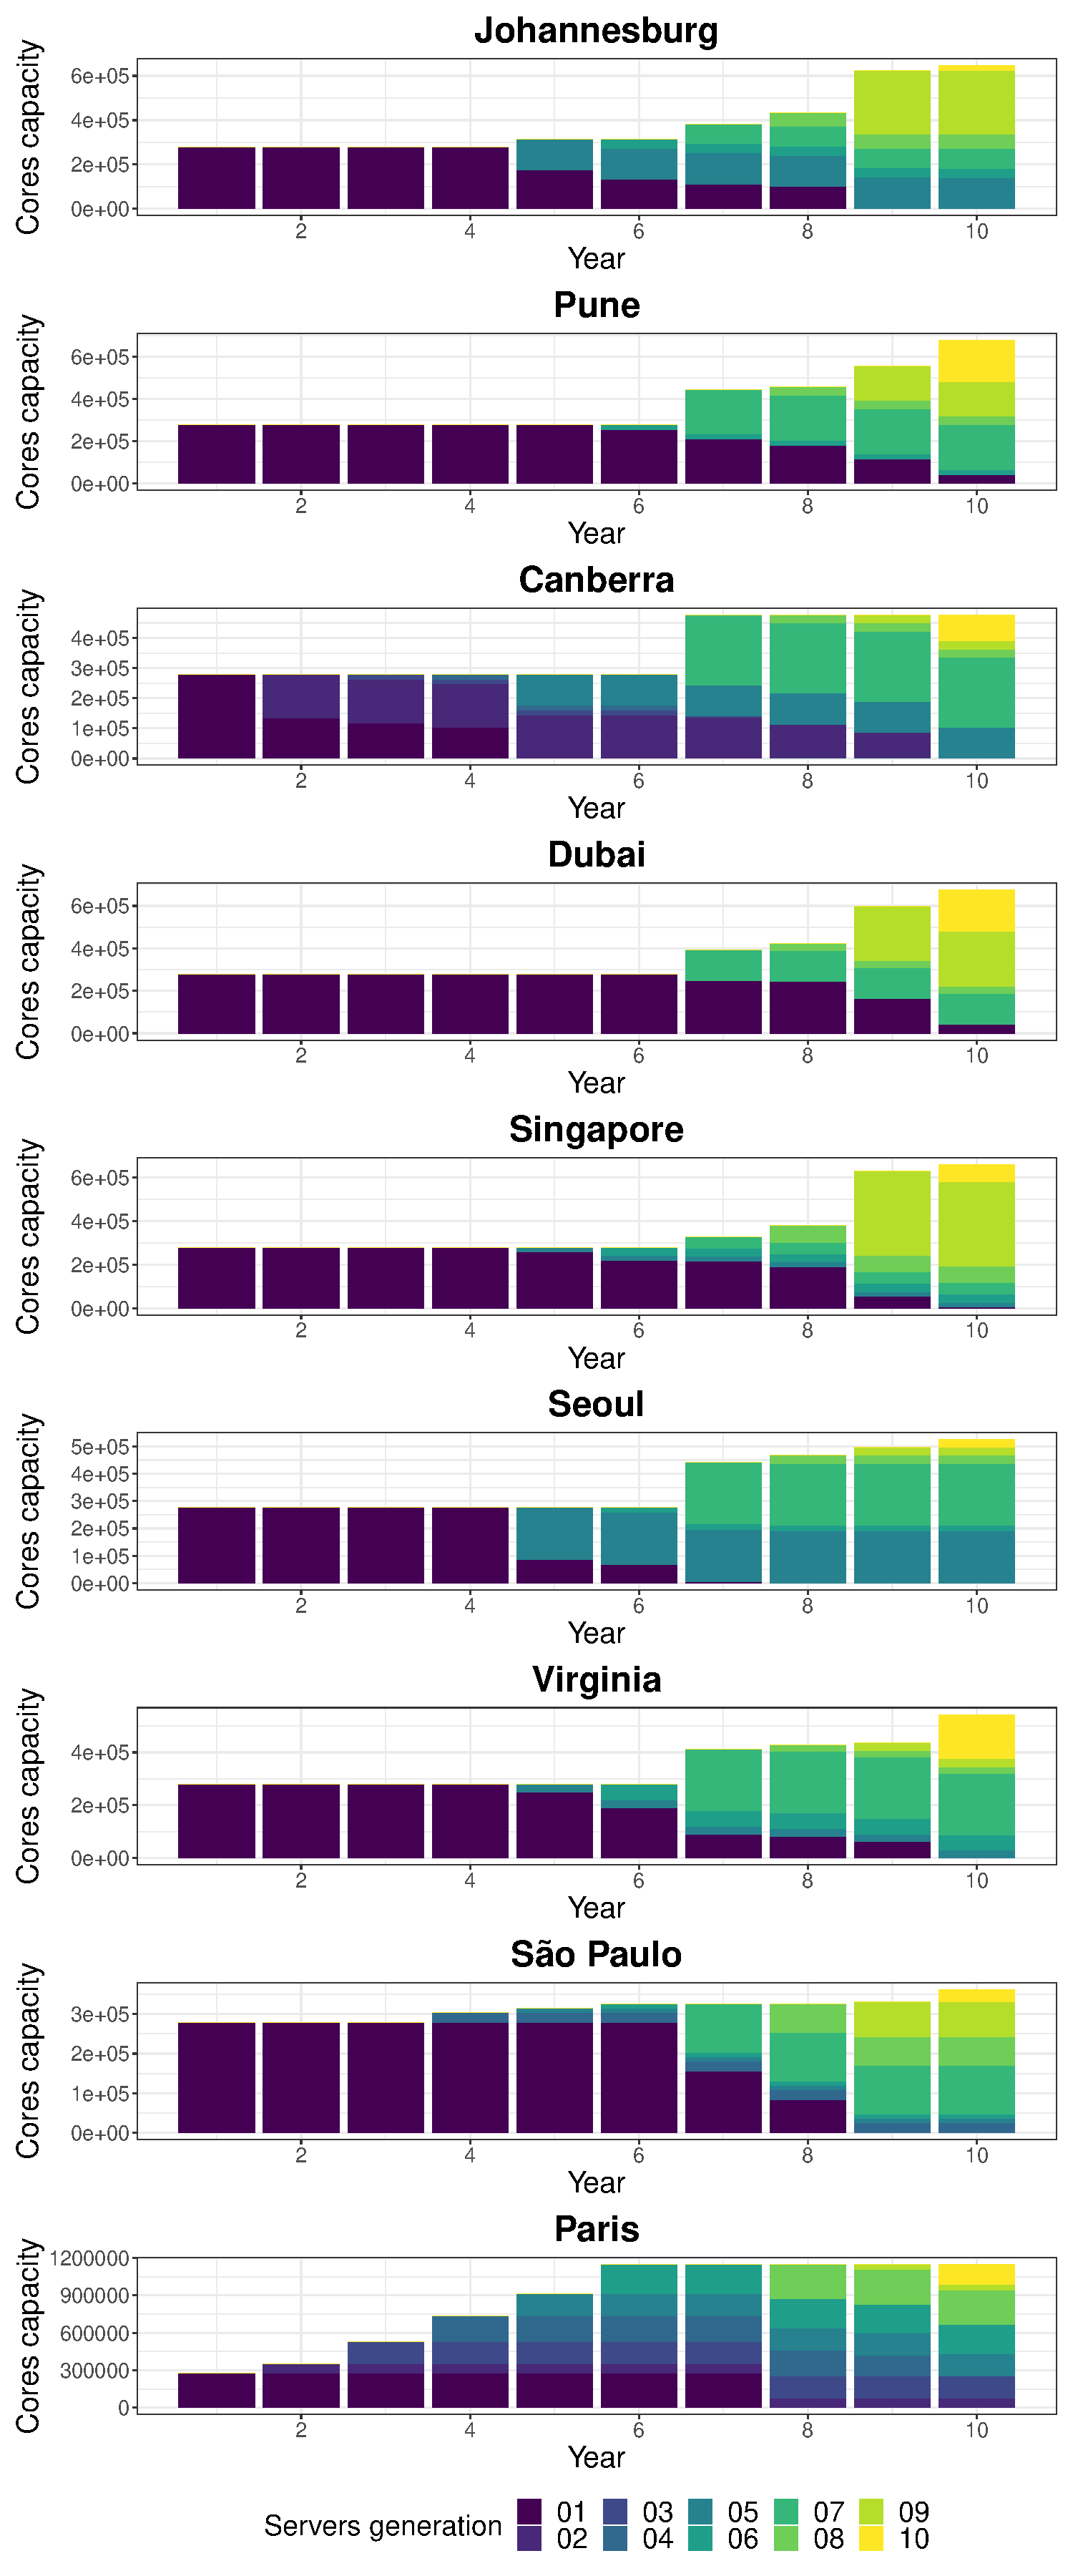
\includegraphics[width=\linewidth]{images/dc_evolution_year_by_year.pdf}
  \caption{Sizing with information of the current year.}
  \label{fig:dc_evolution_year_by_year}
\end{minipage}%
\begin{minipage}{.5\textwidth}
  \centering
  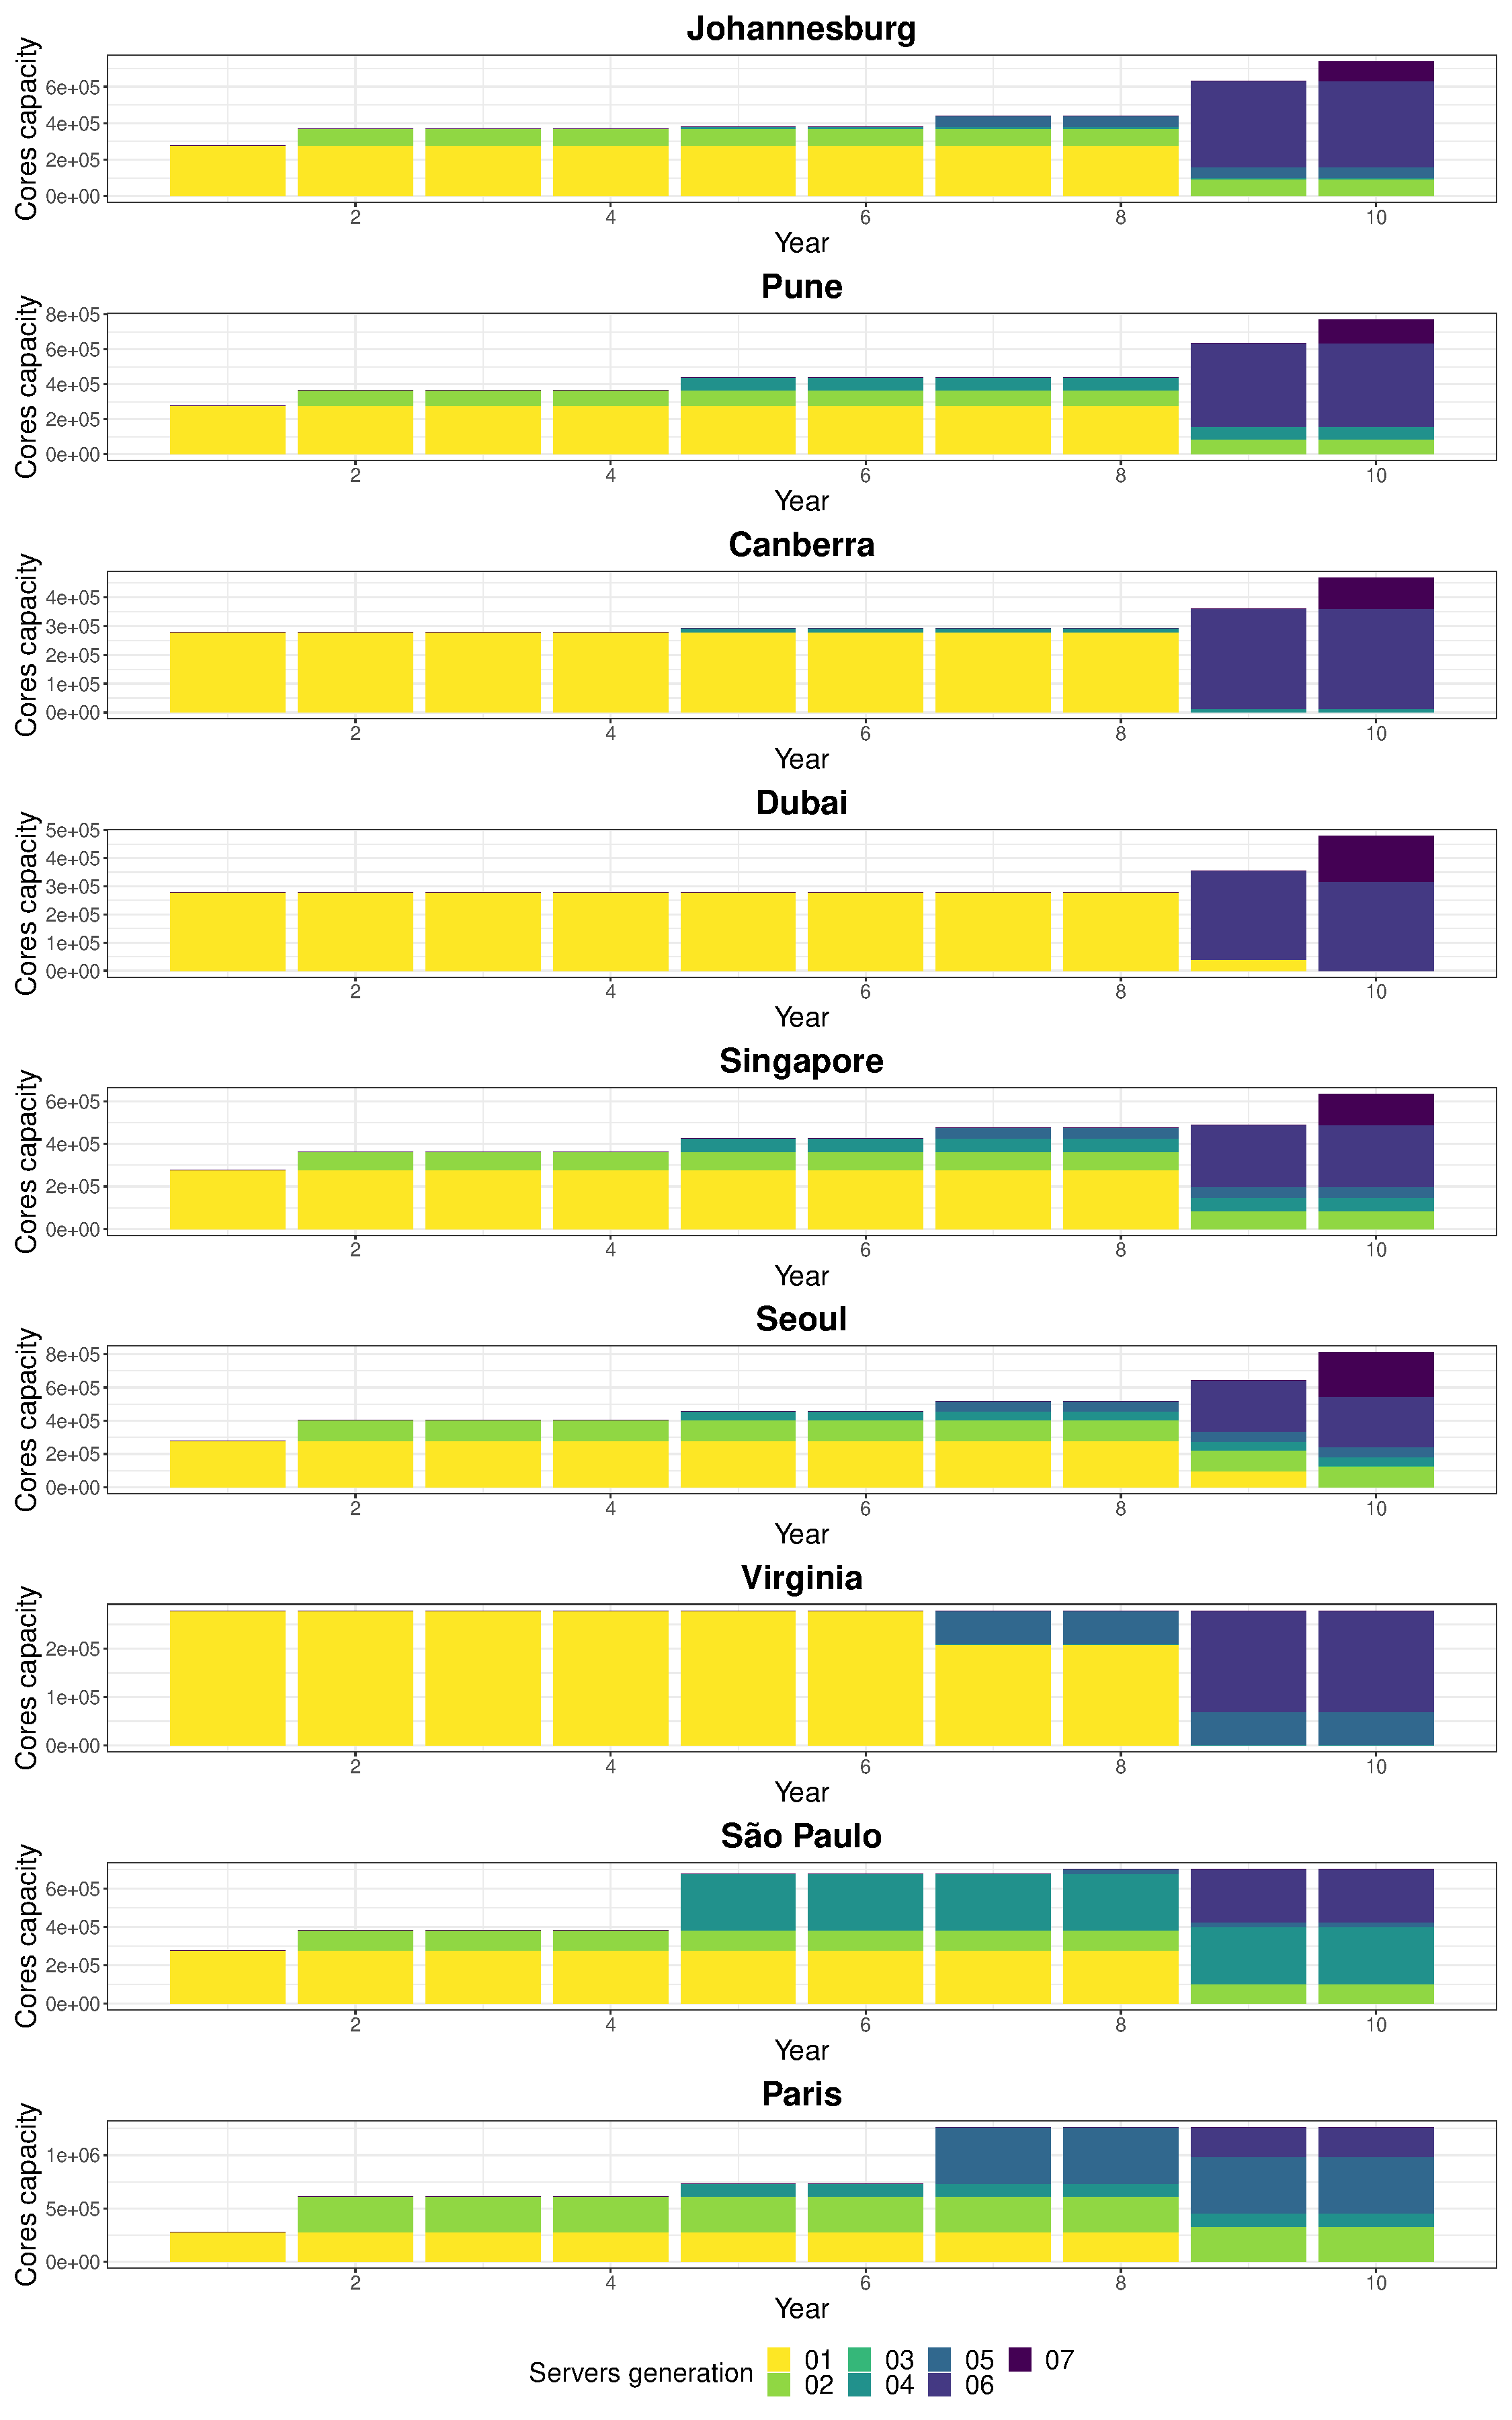
\includegraphics[width=\linewidth]{images/dc_evolution_optimal.pdf}
  \caption{Sizing knowing all information of the 10 years.}
  \label{fig:dc_evolution_optimal}
\end{minipage}
\end{figure}


\subsection{Including degradation in the modeling}

The median of PV modules degradation is around 0.5\% per year \cite{jordan2015_pvdegradationrate}.


\subsection{Evaluating the monetary costs of including renewable infrastructures}

%%% TODOS

%% Add definition of LCOE and LCOS

%%% update objective function to be in terms of price / kwh


In this section, we will evaluate other aspect: the monetary costs in USD of manufacturing the renewable infrastructure and using electricity from the regular electrical grid.  To model this new analysis, we need some modification in our modeling. The first modification regards buying electricity from the regular grid, and it is modeled by Equation~\eqref{eq:pricegrid}, where $costGrid^d$ is an input that represents the costs of buying electricity at each location.  Table~\ref{tab:grid_price} presents the costs of buying electricity from the regular local electricity grid at each location.

\begin{equation} \label{eq:pricegrid}
 PriceGrid^d_k = Pgrid^d_k \times costGrid^d
\end{equation}


\begin{table}[H]
  
  \caption{Local grid electricity price (\$ per kWh) for each location. Source: \url{ https://www.globalpetrolprices.com/electricity_prices/}}\label{tab:grid_price} \centering

  \begin{tabular}{|l|r|}
   \hline
    
  \textbf{Location} &   \textbf{Price} \\
  \hline
  Johannesburg & 0.074   \\
  \hline
  Pune  & 0.104 \\
  \hline
  Canberra  & 0.331 \\
  \hline
  Dubai   &  0.110\\
  \hline
  Singapore & 0.272  \\
  \hline     
  Seoul    & 0.092  \\
  \hline
  Virginia   & 0.150 \\
  \hline
  São Paulo   & 0.144 \\
  \hline 
  Paris    &    0.340 \\
  
  \hline  

\end{tabular}  
\end{table}

Equation~\eqref{eq:pricebat} models the costs of manufacturing batteries, where $costBat$ is an input that represents the costs in \$ per kWh of battery capacity. Here it is considered that the cost per kWh is \$ 153.00 \footnote{Price of battery: \url{https://www.energy.gov/eere/vehicles/articles/fotw-1272-january-9-2023-electric-vehicle-battery-pack-costs-2022-are-nearly}}. Since we consider that the battery lifetime is 10 years, we consider the cost to be \$ 15.30 per year.


\begin{equation} \label{eq:pricebat}
   PriceBat^d = BAT^d \times costBat
\end{equation}

Equation~\eqref{eq:pricepv} models the costs of manufacturing photovoltaic panels, where $costPV$ is an input that represents the costs in \$ per m² of PV area. Here it is considered that building 1 m² PV costs \$ 200.00 \footnote{Price of PVs: \url{ https://www.sunpal-solar.com/info/how-much-does-a-solar-panel-cost-per-square-me-72064318.html}}. Since we consider that the PV lifetime is 30 years, we consider the cost to be \$ 6.66 per year. 


\begin{equation} \label{eq:pricepv}
   PricePV^d = A^d \times costPV
\end{equation}



Equation~\eqref{eq:pricewt} models the costs of manufacturing photovoltaic panels, where $costWT$ is an input that represents the costs in \$ per WT manufactured. Here it is considered that building 1 WT costs \$ 1,950,000\footnote{Price of WTs: \url{https://weatherguardwind.com/how-much-does-wind-turbine-cost-worth-it/}}. Since we consider that the WT lifetime is 20 years, we consider the cost to be \$ 97500 per year. Furthermore, there are also costs for maintenance per year (around \$ 42000); therefore, the final cost is \$ 139500.00 per WT per year.


\begin{equation} \label{eq:pricewt}
PriceWT^d = WT^d \times costWT
\end{equation}

The LP can also be modified in order to minimize the monetary costs in dollars instead of carbon emissions. Equation~\eqref{eq:objective_price} model this new objective.

\begin{equation} \label{eq:objective_price}
\text{minimize }\sum_{k=0}^{K-1} \sum_{d=1}^D PriceGrid^d_k  + \sum_{d=1}^D PriceBat^d + PricePV^d + PriceWT^d
\end{equation}

Table~\ref{tab:total_price} illustrates the total costs for the data center operator considering multiple scenarios. The \textit{Minimum Costs} scenario refers to solving the LP using the objective of Equation~\eqref{eq:objective_price}; the \textit{Minimum \ch{CO2}} refers to solving the LP using  the objective of Equation~\eqref{eq:FPALL}; \textit{Only renewable infra} represents the case where the DC are autonomous and only use power produced from their local renewable infrastructure; and \textit{Only grid} represents the case where there is no renewable infrastructure in the DCs and they only use power from the local electricity grid.


\begin{table}[H]

  \caption{Total costs (millions of \$) for different scenarios }\label{tab:total_price} \centering
  
  \begin{tabular}{|l|r|}
   \hline
    
  \textbf{Scenario} &   \textbf{Total costs (millions of \$)} \\
  \hline
  Minimum cost (PV + Bat + WT + grid) & 36.926   \\
  \hline
  Minimum cost (PV + Bat  + grid)   & 37.889 \\
  \hline
  Minimum \ch{CO2} (PV + Bat + WT + grid)  & 45.667 \\
  \hline
  Minimum \ch{CO2} (PV + Bat + grid)   & 50.054 \\
  \hline
  Only renewable infra (PV + Bat + WT ) & 51.104  \\
  \hline     
  Only renewable infra (PV + Bat)     & 52.694 \\
  \hline
  Only grid   & 75.378\\
  \hline
  
\end{tabular}  
\end{table}


\begin{table}[H]

  \caption{Total emissions (tons of CO2 for different scenarios }\label{tab:total_co2_scenarios} \centering
  
  \begin{tabular}{|l|r|}
   \hline
    
  \textbf{Scenario} &   \textbf{Total CO2 emissions (tons)} \\
  \hline
  Minimum \ch{CO2} (PV + Bat + WT + grid)  & 27821.1\\
  \hline
  Minimum \ch{CO2} (PV + Bat + grid)   & 29541.7 \\
  \hline
  Only renewable infra (PV + Bat)     & 42316.25 \\
  \hline
  Minimum cost (PV + Bat + WT + grid) &  101170.9\\
  \hline
  Minimum cost (PV + Bat  + grid)   & 101930.9 \\
  \hline

\end{tabular}  

\end{table}

\subsection{ Flexibility in the scheduling to reduce carbon emissions}

Suppose that we have the flexibility to delay $\alpha$ percent of workload up to $\beta$ time slots. We need two new variables to model this new feature: $alloc$ that represents the workload allocated that will start executing at the time slot; and $delay$, which represents the workload that can be delayed up to $\beta$ time slots.

This feature also requires the following new restrictions:

\begin{equation} \label{eq:alpha}
   \sum_{d=1}^D  \sum_{i=1}^{\beta} delay_{k,i}^d \leq  \alpha   \times W_k
\end{equation}


Equation~\eqref{eq:alpha} models the flexibility of allowing $\alpha$ percent of the workload to be delayed, where $W_k$ is an input that represents the total workload CPU cores demand to be executed at time slot k.

Equation~\eqref{eq:beta} models the flexibility to delay the workload up to the next $\beta$ time slots and ensure that all the workload will be executed:


\begin{equation} \label{eq:beta}
       \sum_{d=1}^D    (  alloc_k^d +    \sum_{i=1}^{\beta} delay_{k,i}^d  ) = W_k  
\end{equation}

The allocated workload at a time slot k, and the delayed workloads from the previous k - $\beta$ time slots need to respect the data center servers CPU core capacity. Equation ~\eqref{eq:beta_capacity} models this restriction. 

\begin{equation} \label{eq:beta_capacity}
\sum_{d=1}^D    (  alloc_k^d  +    \sum_{i=k-\beta}^{k-1} delay_{  i ,  k-i  }^d  )  \leq C_d 
\end{equation}




  \begin{table}[H]
    \caption{Initial results regarding the relative total carbon emissions reduction (in \%) for different values of $\alpha$ (how much of the workload to delay) and $\beta$ (how long to delay the workload).}\centering
    \label{tab:flex_scheduling}
    \begin{tabular}{|l|r|r|r|r|r|r|r|r|r|r|}
      \hline
      $\alpha$, $\beta$ &   \textbf{$ 1 h $} &   \textbf{$ 6 h $} &  \textbf{$ 12 h $} &  \textbf{$ 24 h $} &  \textbf{$ 48 h $} &  \textbf{$ 96 h$} &   \textbf{$ 120 h $} &   \textbf{$ 144 h$} &   \textbf{$ 168 h$}\\ 
      \hline
      10 \%   &  0.08 &  0.3 &  0.43 &  0.59 &  0.88 &  1.15 &  1.27 &  1.36 &  1.42 \\ 
      \hline
      20 \%   &  0.14 &  0.43 &  0.59 &  0.88 &  1.16 &  1.52 &  1.55 &  1.55 &  1.55 \\ 
      \hline
       30 \%   &  0.19 &  0.51 &  0.75 &  1.04 &  1.38 &  1.55 &  1.55 &  1.56 &  1.56 \\ 
      \hline
       40 \%  &  0.24 &  0.59 &  0.88 &  1.16 &  1.52 &  1.56 &  1.56 &  1.57 &  1.57 \\ 
      \hline
       50 \%   &  0.27 &  0.67 &  0.96 &  1.28 &  1.55 &  1.56 &  1.57 &  1.57 &  1.57 \\ 
      \hline
    \end{tabular}
  \end{table}

In order to evaluate only the impact of the flexibility of the scheduling in reducing the carbon emissions, all the other parameters are fixed: workload, solar irradiation (we used the year 2022), area of PV panels and the capacity of the batteries, power consumption of servers and network devices, and so on. The results of the experiments, when delaying 10\%, 20\%, 30\%, 40\% and 50\% of the workload up to one week (168 hours) are presented in Table \ref{tab:flex_scheduling}.

We can extract two interesting information from the results. The first is that the reduction on the carbon emissions seems to have a limit (1.57\%). This can be justified by the fact that there are no much difference in the climate conditions during the interval of one week, or that the DC which would reduce the carbon emissions is already at peak capacity and cannot receive more workload. The second interesting observation is that by delaying a small portion of the workload (for example 10\% to 20\%)  the reduction is already really close to the maximum value. The reduction in the carbon emissions is low, but it is not negligible, since the order of magnitude of the emissions in a year of the cloud-federation is hundreds of tons of \ch{CO2} eq. Furthermore, it can compensate the impact of the climate conditions intermittency in the sizing, as we in a previous section that the result is up to 2\% far from the optimal.
